\documentclass[10pt,a4paper,twoside]{report}
\usepackage[utf8]{inputenc}

% paquetes usados
\usepackage{tocloft}
\usepackage{tocbibind}
\usepackage{titlesec}
\usepackage[table]{xcolor}
\usepackage{fancyhdr}
\usepackage{tikz-er2}
\usepackage{minted}
\usepackage{pdfpages}
\usepackage{anyfontsize}
\usepackage{wallpaper}
\usepackage{caption}
\usepackage[left=2cm,right=2cm,top=2cm,bottom=2cm]{geometry}

% se definen nuevos colores
\definecolor{azulOscuro}{rgb}{0,0,0.25}
\definecolor{azulMedio}{rgb}{0,0,0.4}
\definecolor{claro}{rgb}{0.9,0.9,0.9}
\definecolor{importante}{rgb}{1,0.4,0.4}
\definecolor{impClaro}{rgb}{1,0.7,0.7}
\definecolor{aclaracion}{rgb}{0,0.9,0.9}
\definecolor{acClaro}{rgb}{0,1,1}
\definecolor{mymauve}{rgb}{0.58,0,0.82}
\definecolor{mygreen}{rgb}{0,0.6,0}

% Configuracion de los captions
\DeclareCaptionFont{azulOscuro}{\color{azulOscuro}}
\captionsetup[figure]{labelfont={azulOscuro,bf,it},textfont={it}}
\captionsetup[table]{labelfont={azulOscuro,bf,it},textfont={it}}

% Se definen nuevos comandos
\newcommand*\circled[1]{\tikz[baseline=(char.base)]{\node[shape=circle,fill=azulOscuro,draw,inner sep=5pt] (char) {#1};}}
\newcommand*\rombo[1]{\tikz[baseline=(char.base)]{\node[shape=diamond,fill=azulOscuro,draw,inner sep=5pt] (char) {#1};}}
\newcommand*\rec[1]{\tikz[baseline=(char.base)]{\node[shape=rectangle,fill=azulOscuro,draw,inner sep=5pt] (char) {#1};}}
\newcommand*\rect[1]{\tikz[baseline=(char.base)]{\node[shape=rectangle,fill=azulMedio,draw,inner sep=5pt] (char) {#1};}}
\newcommand*\elip[1]{\tikz[baseline=(char.base)]{\node[shape=ellipse,fill=azulOscuro,draw,inner sep=5pt] (char) {#1};}}
\newcommand{\bigrule}{\titlerule[0.5mm]}

% Se edita la etiqueta chapter
\titleformat{\chapter} [display]  {\color{azulOscuro}\bfseries\LARGE}
{\vspace*{0.5mm} \filleft {\circled{{\color{white}\Huge\thechapter}}}}
{0mm} {\filleft} [\vspace*{0.5mm}\bigrule]

% Se edita la etiqueta section 
\titleformat{\section} [display]  {\color{azulOscuro}\bfseries\Large}
{\filright {\rec{\color{white}\LARGE\thesection}}}
{0mm} {\filright} []

% Se edita la etiqueta subsection
\titleformat{\subsection} [display]  {\color{azulMedio}\bfseries\large}
{\filright {\rect{\color{white}\Large\thesubsection}}}
{0mm} {\filright} []
 
% Encabezado y pie de pagina
\pagestyle{fancy}
\fancyhead[RE]{}
\fancyhead[RO]{}
\renewcommand{\headrulewidth}{0.5pt}
\fancyfoot[LE,RO]{\rombo{{\color{white}\bfseries\thepage}}}
\fancyfoot[c]{}

% Encabezado y pie de pagina chapter
\fancypagestyle{plain}{
	\fancyhead[L]{}
	\fancyhead[C]{}
	\fancyhead[R]{}
	\fancyfoot[L]{}
	\fancyfoot[C]{}
	\fancyfoot[LE,RO]{\rombo{{\color{white}\bfseries\thepage}}}
	\renewcommand{\headrulewidth}{0pt}
	\renewcommand{\footrulewidth}{0pt}
}

% se renombran comandos
\renewcommand{\abstractname}{Resumen}
\renewcommand{\appendixname}{Apéndice}
\renewcommand{\chaptername}{Capítulo}
\renewcommand{\contentsname}{Contenidos}
\renewcommand{\figurename}{Figura}
\renewcommand{\tablename}{Tabla}
\renewcommand{\cftchapleader}{\cftdotfill{\cftdotsep}}

\author{Juan Luis Navarro}

\usepackage[colorlinks=true,linkcolor=azulOscuro]{hyperref}
\begin{document}
	
	%\maketitle
	{
 \thispagestyle{empty}
 \ThisTileWallPaper{\paperwidth}{\paperheight}{portada/wallpaper.jpg}
 \color{claro}
  
  \setlength{\unitlength}{1 cm} %Especificar unidad de trabajo
  \thispagestyle{empty}
  \vspace*{7cm}
  
  \begin{center}
  	\rule{18cm}{3mm}\\[0.25cm]
  	\textbf{{\fontsize{35}{1}\selectfont Memoria de la aplicación distribuida}\\
  	\rule{18cm}{3mm}\\[0.25cm]}
  	{\fontsize{25}{1}\selectfont Sistemas y Servicios Distribuidos}
  	
  	\vspace{12cm}
  	\raggedleft {\fontsize{17}{1}\selectfont Juan Luis Navarro Rey}
  	
  	
  	
 \end{center}	
}
	
	\begin{abstract}
		Esta es la memoria de la aplicación distribuida mandada en prácticas de la asignatura Sistemas y Servicios Distribuidos. \\ Esta memoria ha sido realizada durante el curso académico 2014/2015.
	\end{abstract}
	
	\tableofcontents
	\thispagestyle{empty}
	
	\chapter{Introducción}
Esta aplicación consiste en sincronizar dos directorios. Un directorio en un cliente y otro en un servidor. Si el fichero que se encuentra en el cliente no existe en el directorio del servidor, entonces el cliente subirá el fichero al servidor. Si el fichero que se encuentra en el servidor no existe en el cliente, entonces el cliente se descargará del servidor dicho fichero. \\ \\ Para implementar la aplicación se va a usar java rmi. La aplicación constará de tres partes:
\begin{itemize}
	\item Servidor
	\item Proxy
	\item Cliente
\end{itemize}

\section{Java RMI}
RMI (Java Remote Method Invocation) es un mecanismo ofrecido por Java para invocar un método de manera remota. Forma parte del entorno estándar de ejecución de Java y proporciona un mecanismo simple para la comunicación de servidores en aplicaciones distribuidas basadas exclusivamente en Java. Si se requiere comunicación entre otras tecnologías debe utilizarse CORBA o SOAP en lugar de RMI.\\
RMI se caracteriza por la facilidad de su uso en la programación por estar específicamente diseñado para Java; proporciona paso de objetos por referencia (no permitido por SOAP), recolección de basura distribuida (Garbage Collector distribuido) y paso de tipos arbitrarios (funcionalidad no provista por CORBA).

\section{Servidor}
Se ha diseñado el servidor como una aplicación de consola ya que no tiene sentido crear una interfaz gráfica ya que el cliente hará una petición al servidor mediante el proxy al servidor. El servidor ejecutará la petición y devolverá al cliente el resultado mediante el proxy.

\section{Proxy}
El proxy es una interfaz en la cual tiene definidas las cabeceras de las funciones del servidor. El proxy es el encargado de hacer posible la comunicación entre el cliente y el servidor dando transparencia al cliente.

\section{Cliente}
Se ha diseñado el cliente con una interfaz gráfica para simplificar el manejo de la aplicación distribuida al cliente. Cuando el cliente desea realizar una petición al servidor, éste invoca al proxy y el proxy realiza la petición al servidor. Cuando el servidor acaba, el resultado le llega al cliente mediante el proxy.

\section{Configuración}
Para configurar correctamente RMI es necesario cumplir los siguientes pasos:
\begin{enumerate}
	\item Crear el fichero server.policy
	\item Es necesario pasar parámetros a la máquina virtual java.
\end{enumerate}
\subsection{Configuración del fichero server.policy}
Este fichero contiene la configuración de permisos de acceso. Para dar correctamente hay que crear el fichero server.policy con el siguiente código.\\
\inputminted[bgcolor=claro]{RobotFramework}{/home/juan/IdeaProjects/ficherormi/target/classes/server.policy}
\subsection{Configuración de la máquina virtual}
Una vez creado el fichero server.policy hay que pasar los siguientes parámetros a la máquina virtual.
\begin{enumerate}
	\item -Djava.rmi.server.codebase=file://$<$ruta$>$ 
	\item -Djava.security.policy=file://$<$ruta$>$server.policy
\end{enumerate}
En el primer parámetro se indica la ruta de los ficheros binarios de la aplicación. En el segundo parámetro se indica la ruta del fichero server.policy

	
	\chapter{Servidor}
\section{Introducción}
Se ha diseñado el servidor como una aplicación de consola ya que no tiene sentido crear una interfaz gráfica ya que el cliente hará una petición al servidor mediante el proxy al servidor. El servidor ejecutará la petición y devolverá al cliente el resultado mediante el proxy.

\section{Funcionalidad del servidor}
El servidor tiene las siguientes funcionalidades: descargar fichero, dar la hora que tiene, lista los ficheros de la carpeta remota, cambiar el directorio remoto, subir un fichero y por último devolver la última modificación de un fichero.

\subsection{Descargar fichero}
Descarga un fichero sin tener en cuenta la fecha de la última modificación. Si se quiere tener en cuenta la fecha de la última modificación, hay que comprobar previamente que el fichero del cliente es más viejo que el del servidor.
\\
Este método descarga un fichero mediante un buffer de bytes el cual se envía al cliente. Se realiza de esta manera para optimizar el uso de la aplicación. Los parámetros que acepta el método son los siguientes:
\begin{itemize}
	\item name: Nombre del fichero que se quiere descargar.
	\item index: Se empieza a llenar el buffer, el cual se va a enviar al cliente, en el byte número index del texto que contiene el fichero que se quiere descargar.
\end{itemize}
Lo primero que hace el método es comprobar que el fichero que se quiere descargar existe en la carpeta del servidor. Si no existe se manda un mensaje de error al cliente.\\ A continuación se calcula el número de la iteración, es decir, cuantos buffers (partes) se le han mandado ya al cliente. Se utiliza el número de iteración para saber si en la iteración actual se va a rellenar el buffer. Si es así crea el buffer con la longitud habitual. De no rellenarse el buffer, se calcula el número de bytes que se van a mandar al cliente y se crea el buffer con dicha longitud.\\ Una vez rellenado el buffer se calcula si en la iteracción actual se completa el fichero. Si es así, al final del buffer se manda un carácter de escape seguido de la cadena `FIN'. De no completarse el fichero en la iteración actual, al final del buffer se manda un carácter de escape seguido de la cadena `continue' para que el cliente sepa que tiene que mandar una nueva petición al servidor.

\subsection{Devolver la hora}
El servidor accede al reloj del sistema operativo, captura la hora y la traduce en milisegundos. A continuación, se la envía al cliente si no se produce ningún error. En el caso de que se produzca un error en alguna operación le envía el servidor al cliente un mensaje de error.

\subsection{Listar ficheros}
Este método se encarga de averiguar el nombre de todos los ficheros que se encuentran en la carpeta remota.

\subsection{Modificar la carpeta remota del servidor}
Para implementar esta función se han generado dos métodos en el servidor. El primero, no tiene parámetros y lista los posibles directorios remotos del servidor y se los envía al cliente. El cliente elige el directorio remoto del servidor y llama al segundo método que coge como parámetro la ruta del directorio. Este segundo método, coge la ruta pasada como parámetro y le asocia la carpeta remota.

\subsection{Subir fichero}
Sube un fichero sin tener en cuenta la fecha de la última modificación. Si se quiere tener en cuenta la fecha de la última modificación, hay que comprobar previamente que el fichero del cliente es más nuevo que el del servidor.
\\
Este método sube un fichero mediante un buffer de bytes el cual se envía al servidor. Se realiza de esta manera para optimizar el uso de la aplicación. Los parámetros que acepta el método son los siguientes:
\begin{itemize}
	\item name: Nombre del fichero que se quiere subir.
	\item buffer: Parte del fichero que se va a subir al servidor.
	\item actualizar: Vale true si se va a actualizar el fichero y por tanto hay que borrar el fichero existente.
\end{itemize}
Lo primero que hace el método es comprobar que el fichero que se quiere subir existe.  Si no existiese, el servidor lo crea.\\ Lo siguiente es comprobar si la parte enviada es la primera parte o no. Si es la primera parte, entonces el parámetro actualizar vale true. Si no es la primera parte, entonces se lee el contenido del fichero y se guarda en una variable.\\ Después, se añade a la variable auxiliar el buffer de contenido enviado por el cliente.\\ A continuación, se comprueba que el fichero que se quiere escribir tiene permisos de escritura. Si no los tiene, se manda un mensaje de error al cliente. Si se puede escribir, entonces se escribe en el fichero.

\subsection{Última modificación}
Averigua la última modificación de un fichero.
Este método acepta el siguiente parámetro:
\begin{itemize}
	\item nombre: Nombre del fichero que se quiere saber la última modificación.
\end{itemize}
Lo primero que hace es comprobar si el fichero existe. Si el fichero no existe, se manda un mensaje de error al cliente. Si existe el fichero, se calculará la última modificación y se enviará al cliente.
	
	\chapter{Proxy}
\section{Introducción}
El proxy es una interfaz en la cual tiene definidas las cabeceras de las funciones del servidor. El proxy es el encargado de hacer posible la comunicación entre el cliente y el servidor dando transparencia al cliente.

\section{Funcionalidad}
El proxy contiene las siguientes funciones (métodos):
\begin{table}[h!]
	\centering
	\rowcolors{1}{white}{claro}
	\setlength\arrayrulewidth{1.2pt}
	\begin{tabular}{p{7cm} @{\hspace{3mm}}p{8cm}}
		\hline Función & Descripción\\
		\hline descargarFichero(java.lang.String name, int index) & Sube un fichero a la carpeta remota.\\
		getHoraServidor() & El servidor calcula la hora que tiene y la devuelve en milisegundos\\
		listaFicherosCarpetaRemota() & Crea una lista con el nombre de todos los ficheros que existen el la carpeta remota
		del servidor\\
		modificaCarpetaServidor() & Modifica la carpeta remota del servidor\\
		modificaCarpetaServidor(java.lang.String carpetaServidor) & Modifica la carpeta remota del servidor\\
		subirFichero(java.lang.String name, byte[] contenido,boolean actualizar) & Sube un fichero a la carpeta remota\\
		ultimaModificacion(java.lang.String nombre) & Averigua la ultima modificacion de un fichero\\
		\hline
	\end{tabular}
	\caption{Funcionalidad del proxy}
	\label{tabla:funcionalidad_proxy}
\end{table}
\\
Para ver la documentación con más detalle, ver la sección \ref{javadoc}.
	
	\chapter{Cliente}
\section{Introducción}
Se ha diseñado el cliente con una interfaz gráfica para simplificar el manejo de la aplicación distribuida al cliente. Cuando el cliente desea realizar una petición al servidor, éste invoca al proxy y el proxy realiza la petición al servidor. Cuando el servidor acaba, el resultado le llega al cliente mediante el proxy.

\section{Ejecución de la aplicación}
Una vez que se ejecuta la aplicación, lo primero que pide es la IP del servidor tal y como se ve en la figura \ref{fig:elegir_ip}
\begin{figure}[htb]
	\centering
	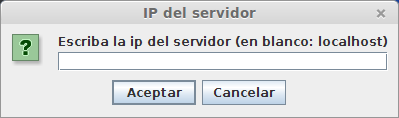
\includegraphics[scale=1]{imagenes/elegir_ip.png}
	\caption{Elegir IP}
	\label{fig:elegir_ip}
\end{figure}
Una vez introducida la IP se ejecuta la ventana principal de la aplicación.

\subsection{Ventana principal}
La ventana principal (ver figura \ref{fig:main_gui}) consta de una barra de menú y de cuatro botones:
\begin{itemize}
	\item Subir fichero: sube un fichero al servidor.
	\item Descargar fichero: descarga un fichero al cliente.
	\item Sincronizar reloj: Sincroniza el reloj del cliente con el del servidor.
	\item Actualizar directorios: Actualiza los directorios (remoto y local).
\end{itemize}

\begin{figure}[htb]
	\centering
	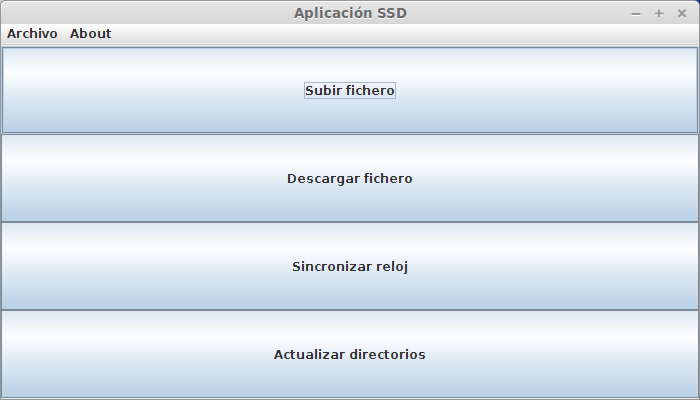
\includegraphics[scale=0.7]{imagenes/main_gui.png}
	\caption{Ventana principal}
	\label{fig:main_gui}
\end{figure}

\hspace*{-5mm} El contenido de la barra de menú es el siguiente:
\begin{itemize}
	\item Archivo
	\begin{itemize}
		\item Ajuestes
		\begin{itemize}
			\item Cambiar carpeta local: cambia la carpeta local
			\item Cambiar carpeta remota: cambia la carpeta remota (ver figura \ref{fig:remote_folder_gui})
			\item Cambiar Tmin: cambia el tiempo mínimo de transmisión de un paquete del cliente al servidor
		\end{itemize}
		\item Salir: cierra la aplicación
	\end{itemize}
	\item About
	\begin{itemize}
		\item Carpeta local: muestra la ruta de la carpeta local.
		\item Tmin: muestra el valor del tiempo mínimo de transmisión de un paquete del cliente al servidor
		\item Información: muestra la información acerca de la aplicación
	\end{itemize}
\end{itemize}

\begin{figure}[htb]
	\centering
	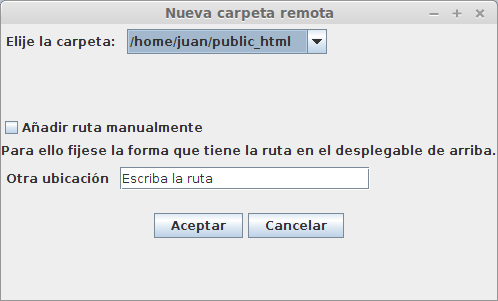
\includegraphics[scale=0.7]{imagenes/remote_folder_gui.png}
	\caption{Elegir directorio remoto}
	\label{fig:remote_folder_gui}
\end{figure}

\subsection{Elegir directorio remoto}
Como se puede observar en la figura \ref{fig:remote_folder_gui}, la ventana consta de dos partes.\\ La primera parte contiene un desplegable con todas las posibles carpetas (existentes) del servidor que pueden ser la nueva carpeta remota.
\\Si por algún motivo se quisiese elegir otra carpeta en la segunda parte se ha creado un campo de texto para introducir la ruta. \\Cuando se le da al botón de aceptar, por defecto escoge la ruta de la primera parte. Si se quiere poner una ruta manualmente es necesario activar la casilla que hay justo encima para que la ruta que se pase al servidor sea la ruta manual.

	
	\appendix 
\chapter{Documentación de la aplicación distribuida}
\section{Javadoc}
Javadoc es una utilidad de Oracle para la generación de documentación de APIs en formato HTML a partir de código fuente Java. Javadoc es el estándar de la industria para documentar clases de Java. La mayoría de los IDEs los generan automáticamente.\\ \\
A continuación se explican algunas de las palabras reservadas:
\begin{table}[h!]
	\centering
	\rowcolors{1}{white}{claro}
	\setlength\arrayrulewidth{1.2pt}
	\begin{tabular}{p{4cm} @{\hspace{1mm}}p{9cm}}
		\hline Tag & Descripción\\
		\hline @author & Nombre del desarrollador\\
		@deprecated & Indica que el método o clase es antigua y que no se recomienda su uso porque posiblemente desaparecerá en versiones posteriores\\
		@param & Definición de un parámetro de un método, es requerido para todos los parámetros del método\\
		@return & Informa de lo que devuelve el método, no se puede usar en constructores o métodos "void"\\
		@see & Asocia con otro método o clase\\
		@throws & Excepción lanzada por el método\\
		@version & Versión del método o clase\\
		\hline
	\end{tabular}
	\caption{Uso de los tags}
	\label{tabla:formato_javadoc}
\end{table}

\section{Documentación}
\label{javadoc}
En las siguientes páginas se puede ver la documentación de la aplicación.
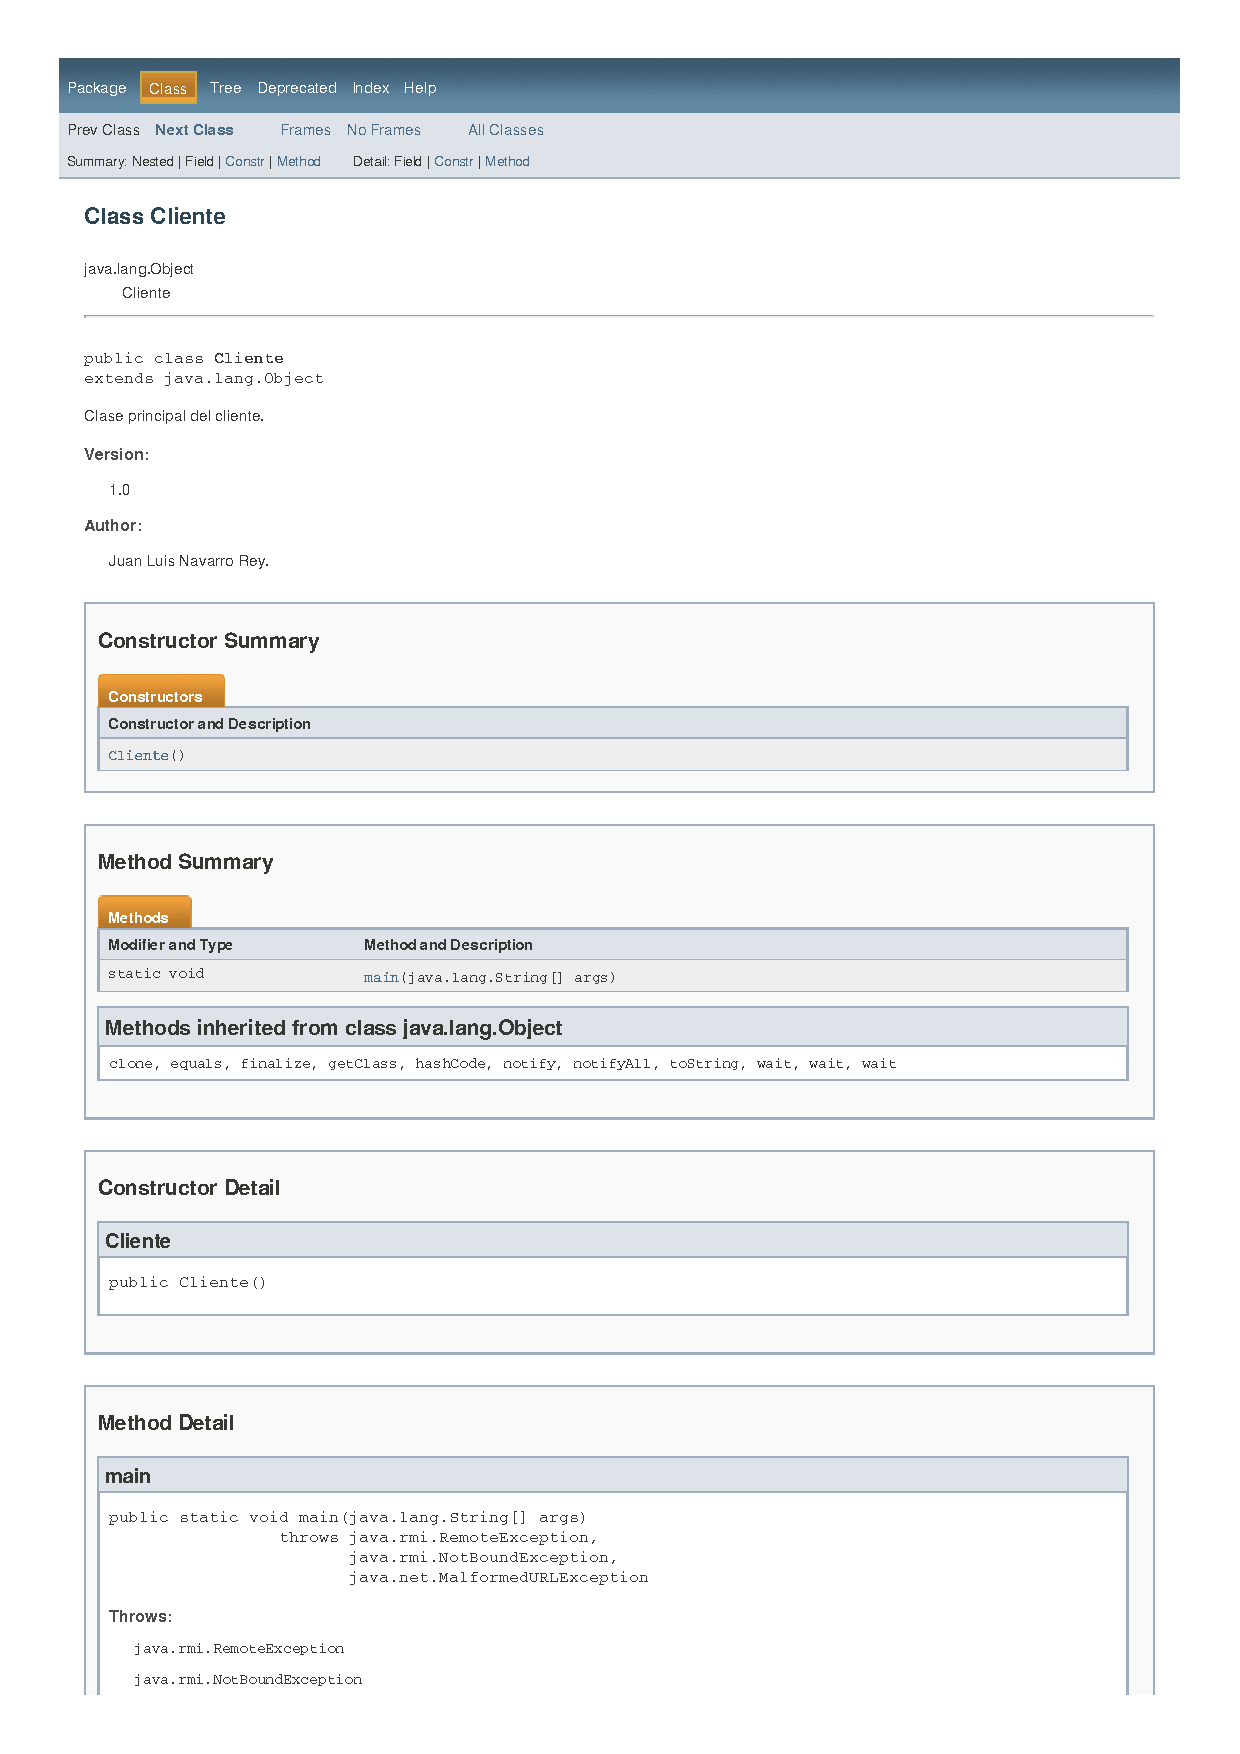
\includepdf[pages=-,nup=1x1,frame=false,scale=0.9,pagecommand={\label{doc:cliente}}]{javadoc/Cliente.pdf}
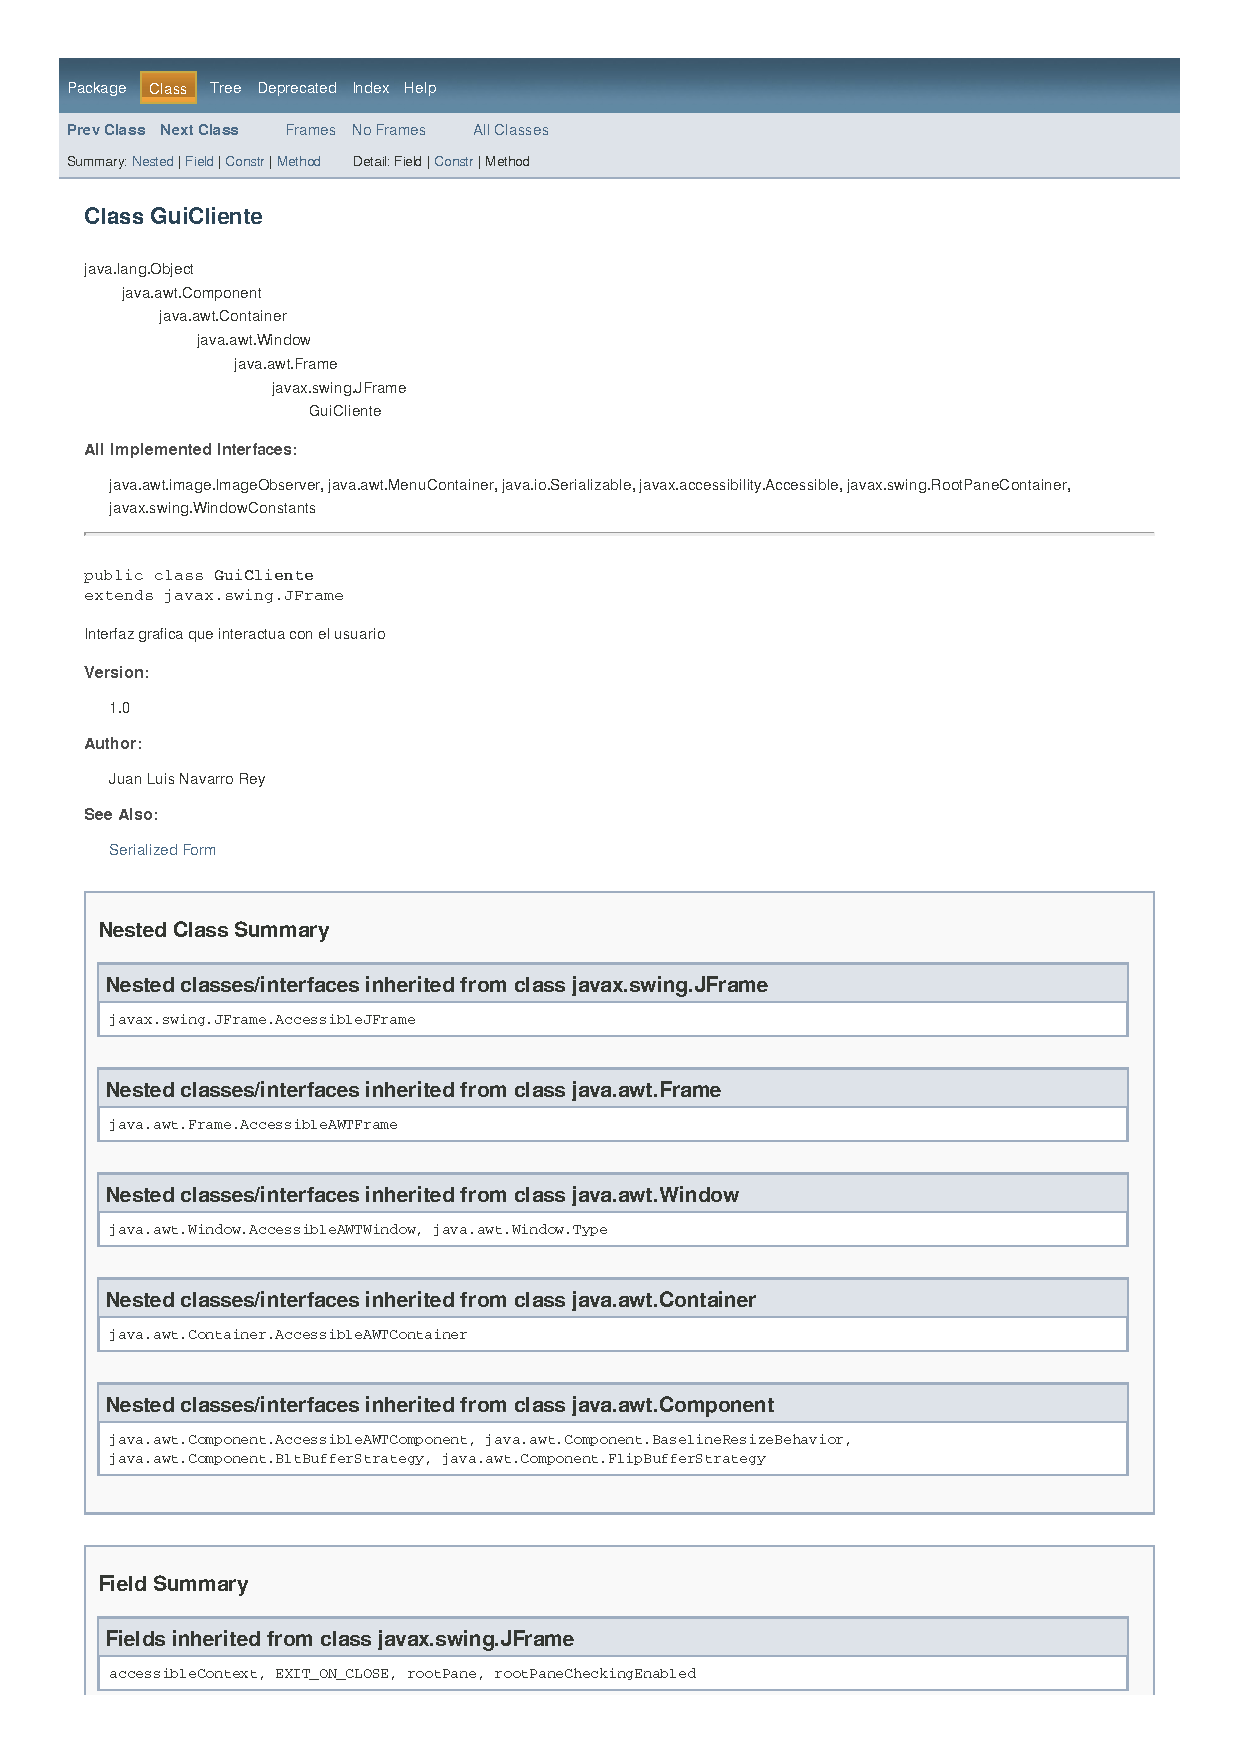
\includepdf[pages=-,nup=1x1,frame=false,scale=0.9,pagecommand={\label{doc:guicliente}}]{javadoc/GuiCliente.pdf}
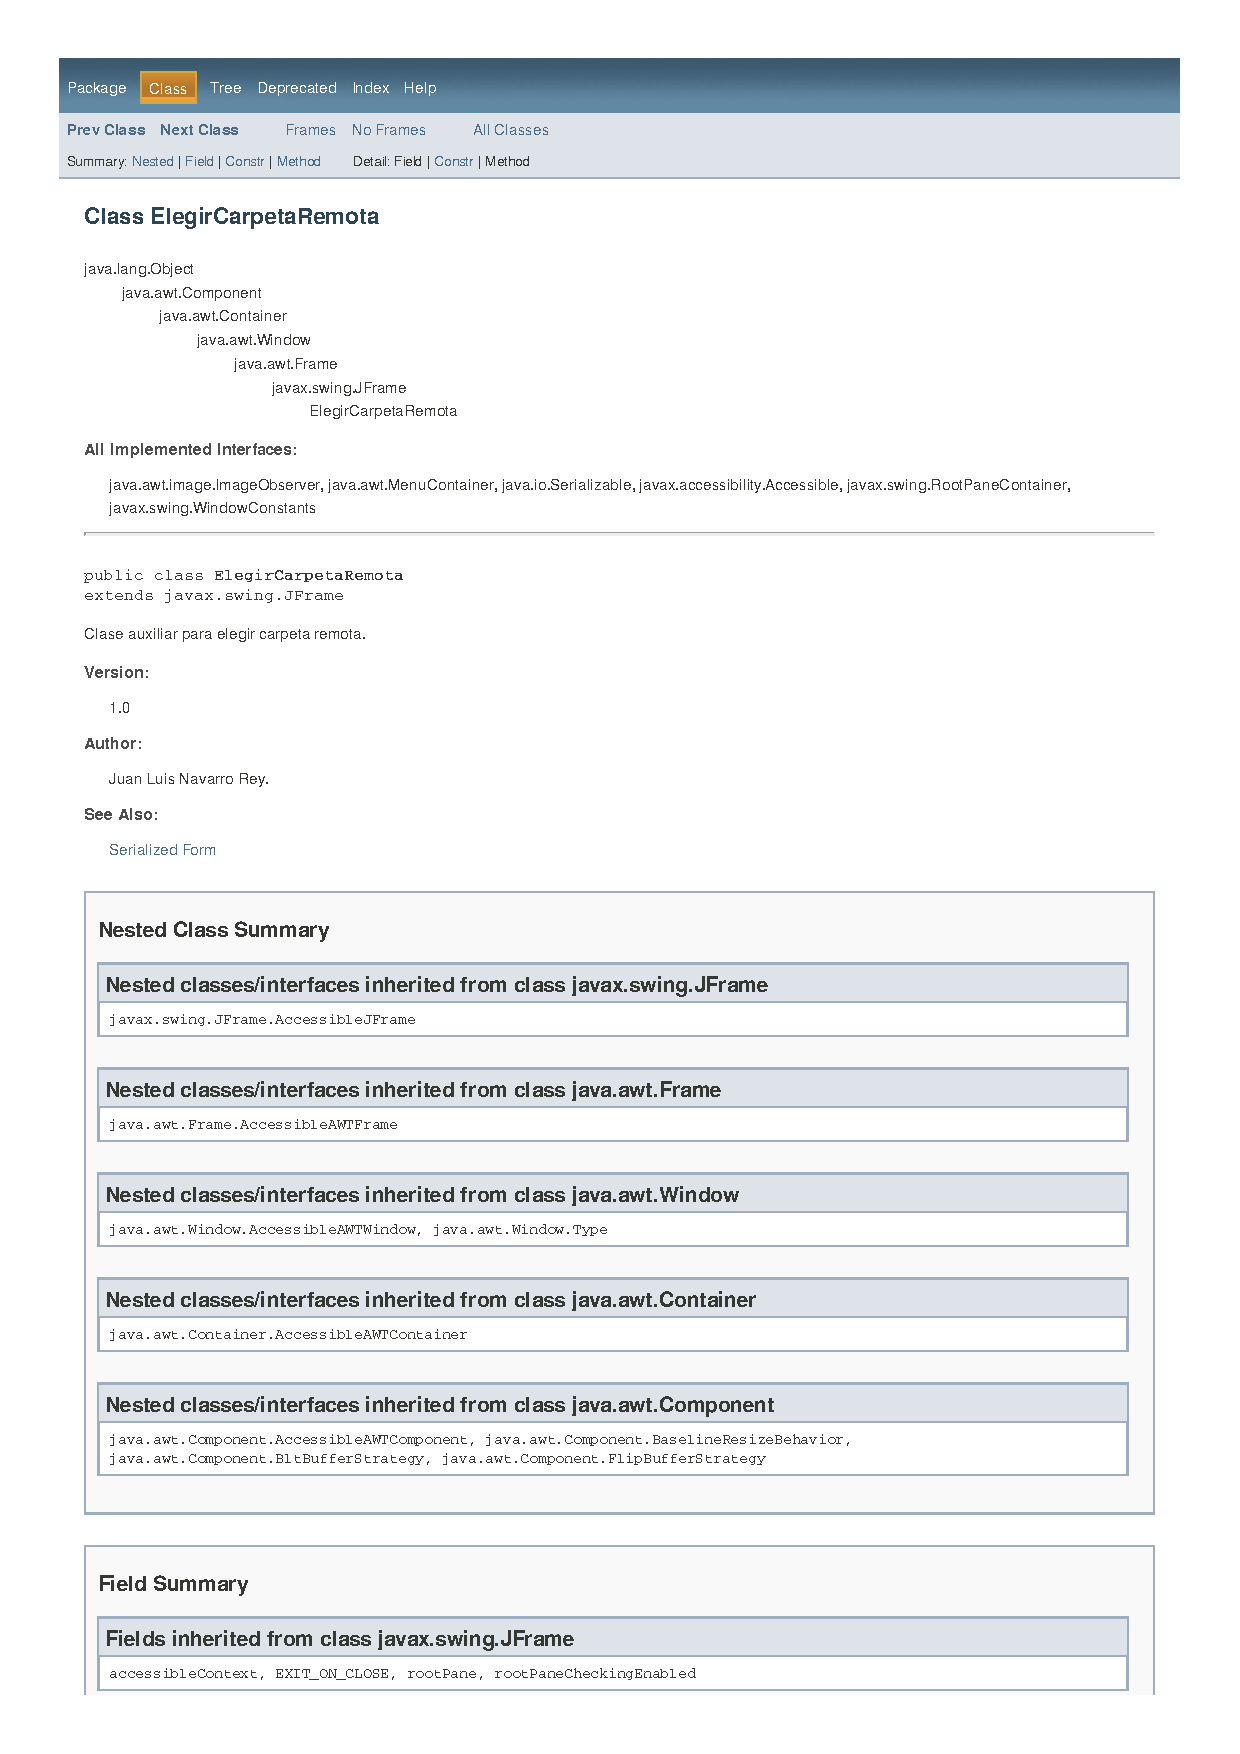
\includepdf[pages=-,nup=1x1,frame=false,scale=0.9,pagecommand={\label{doc:elegircarpetaremota}}]{javadoc/ElegirCarpetaRemota.pdf}
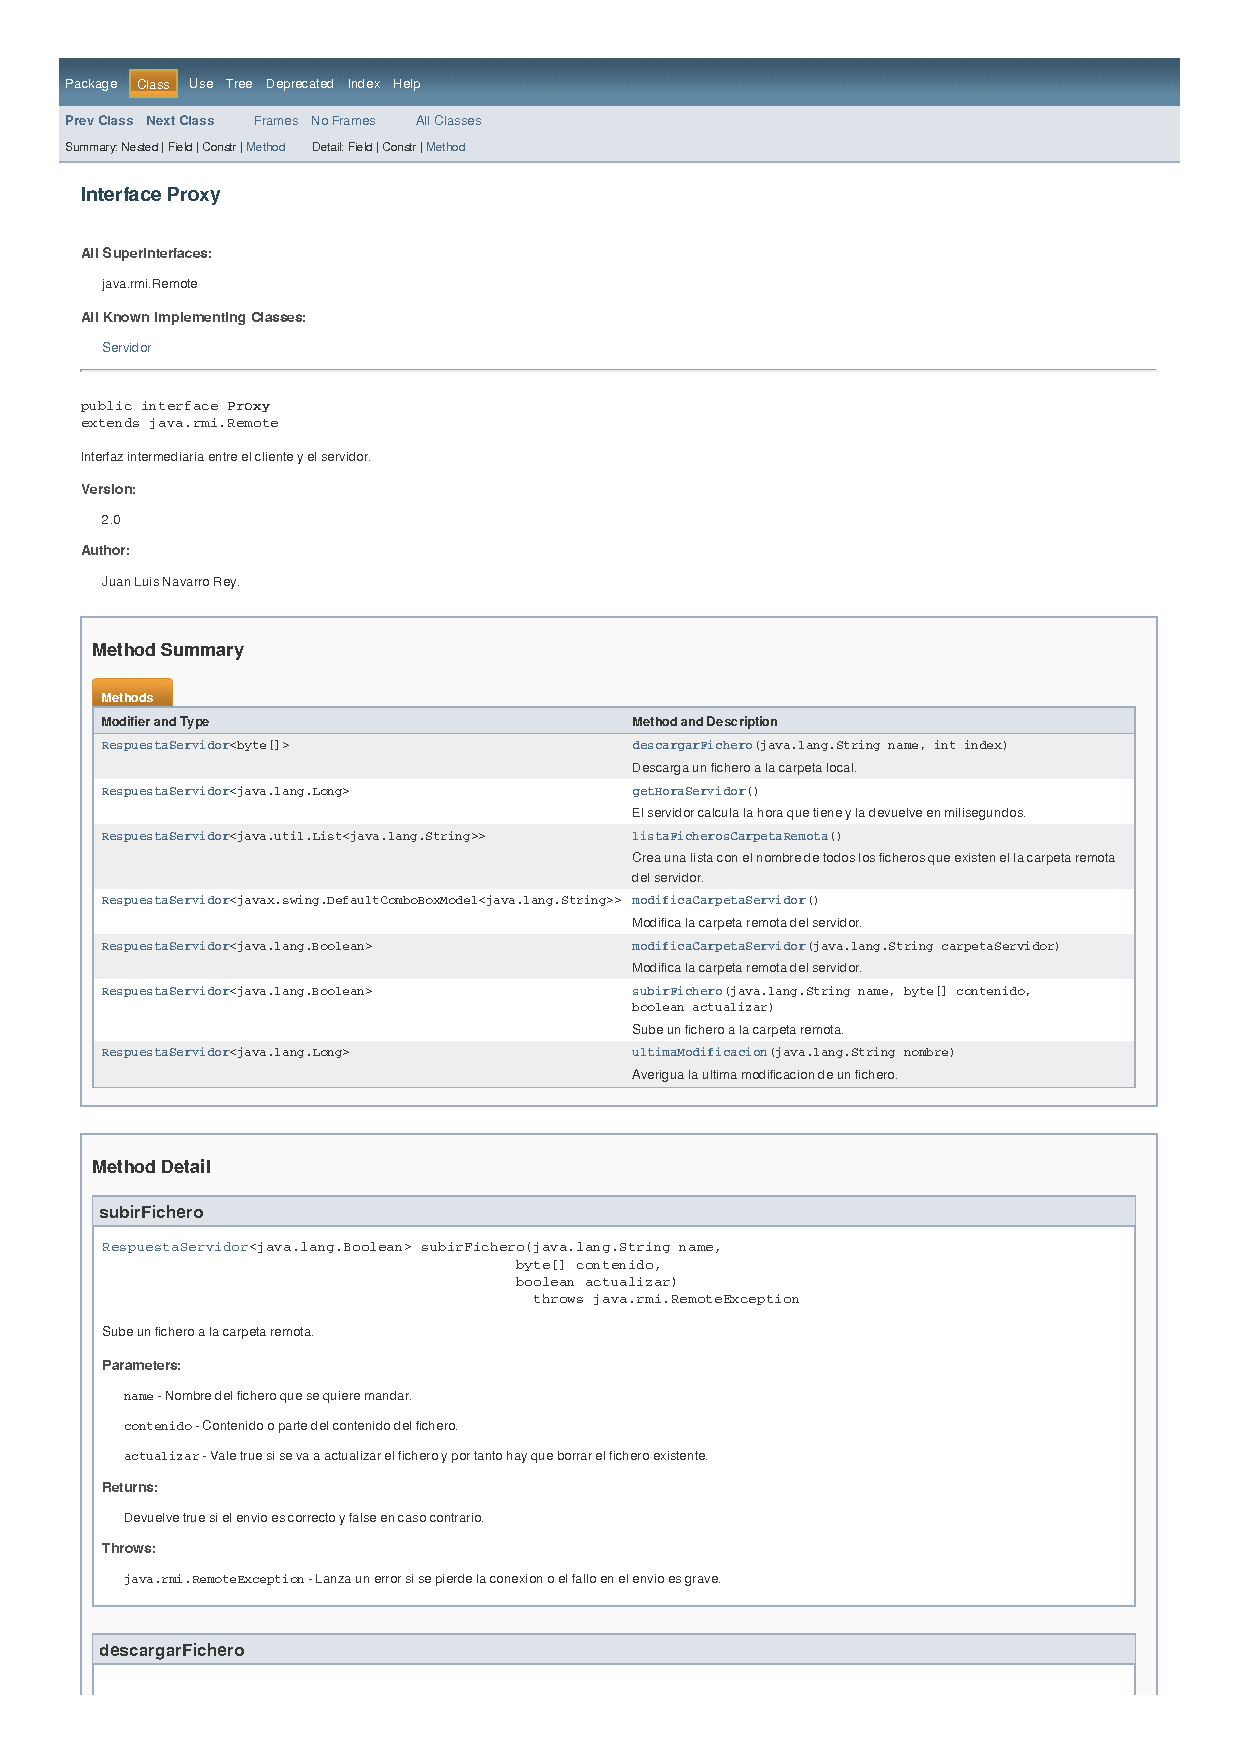
\includepdf[pages=-,nup=1x1,frame=false,scale=0.9,pagecommand={\label{doc:proxy}}]{javadoc/Proxy.pdf}
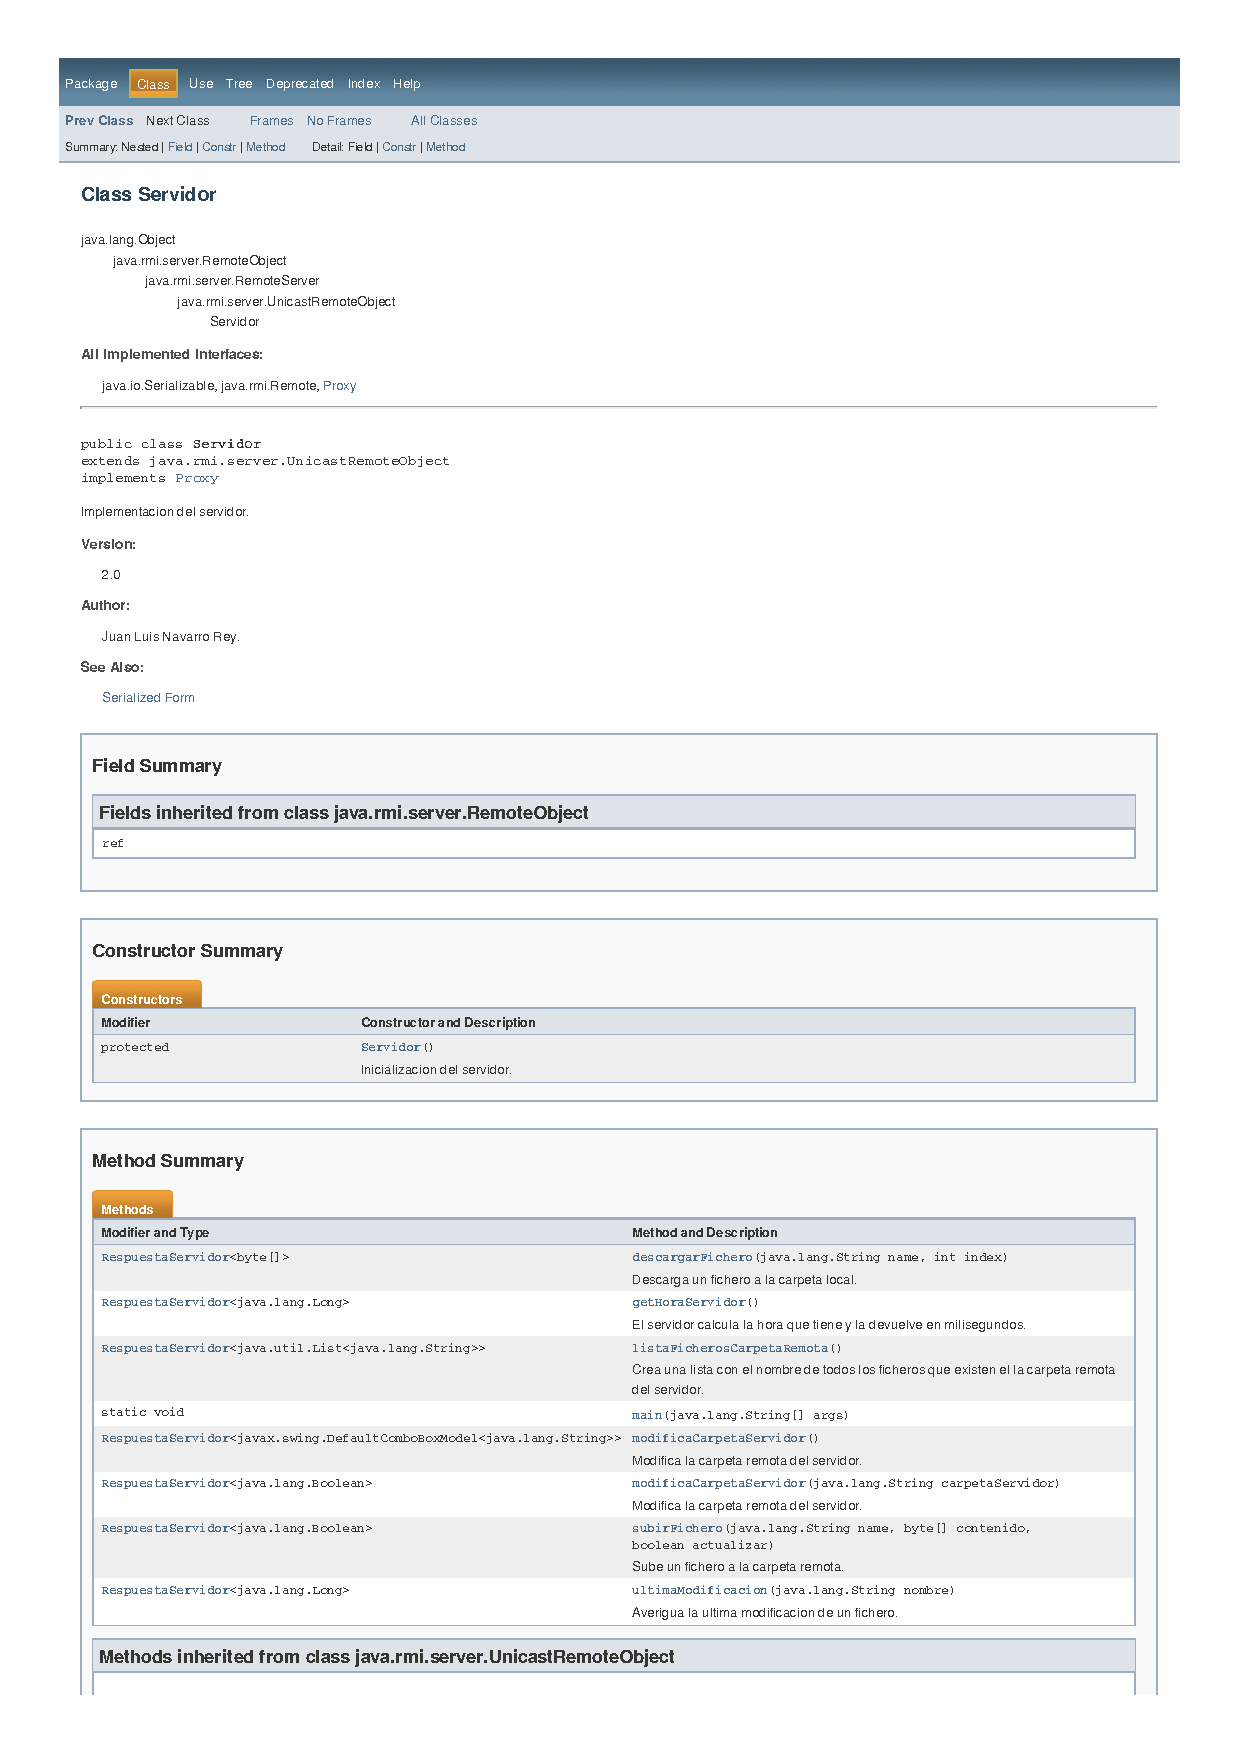
\includepdf[pages=-,nup=1x1,frame=false,scale=0.9,pagecommand={\label{doc:servidor}}]{javadoc/Servidor.pdf}
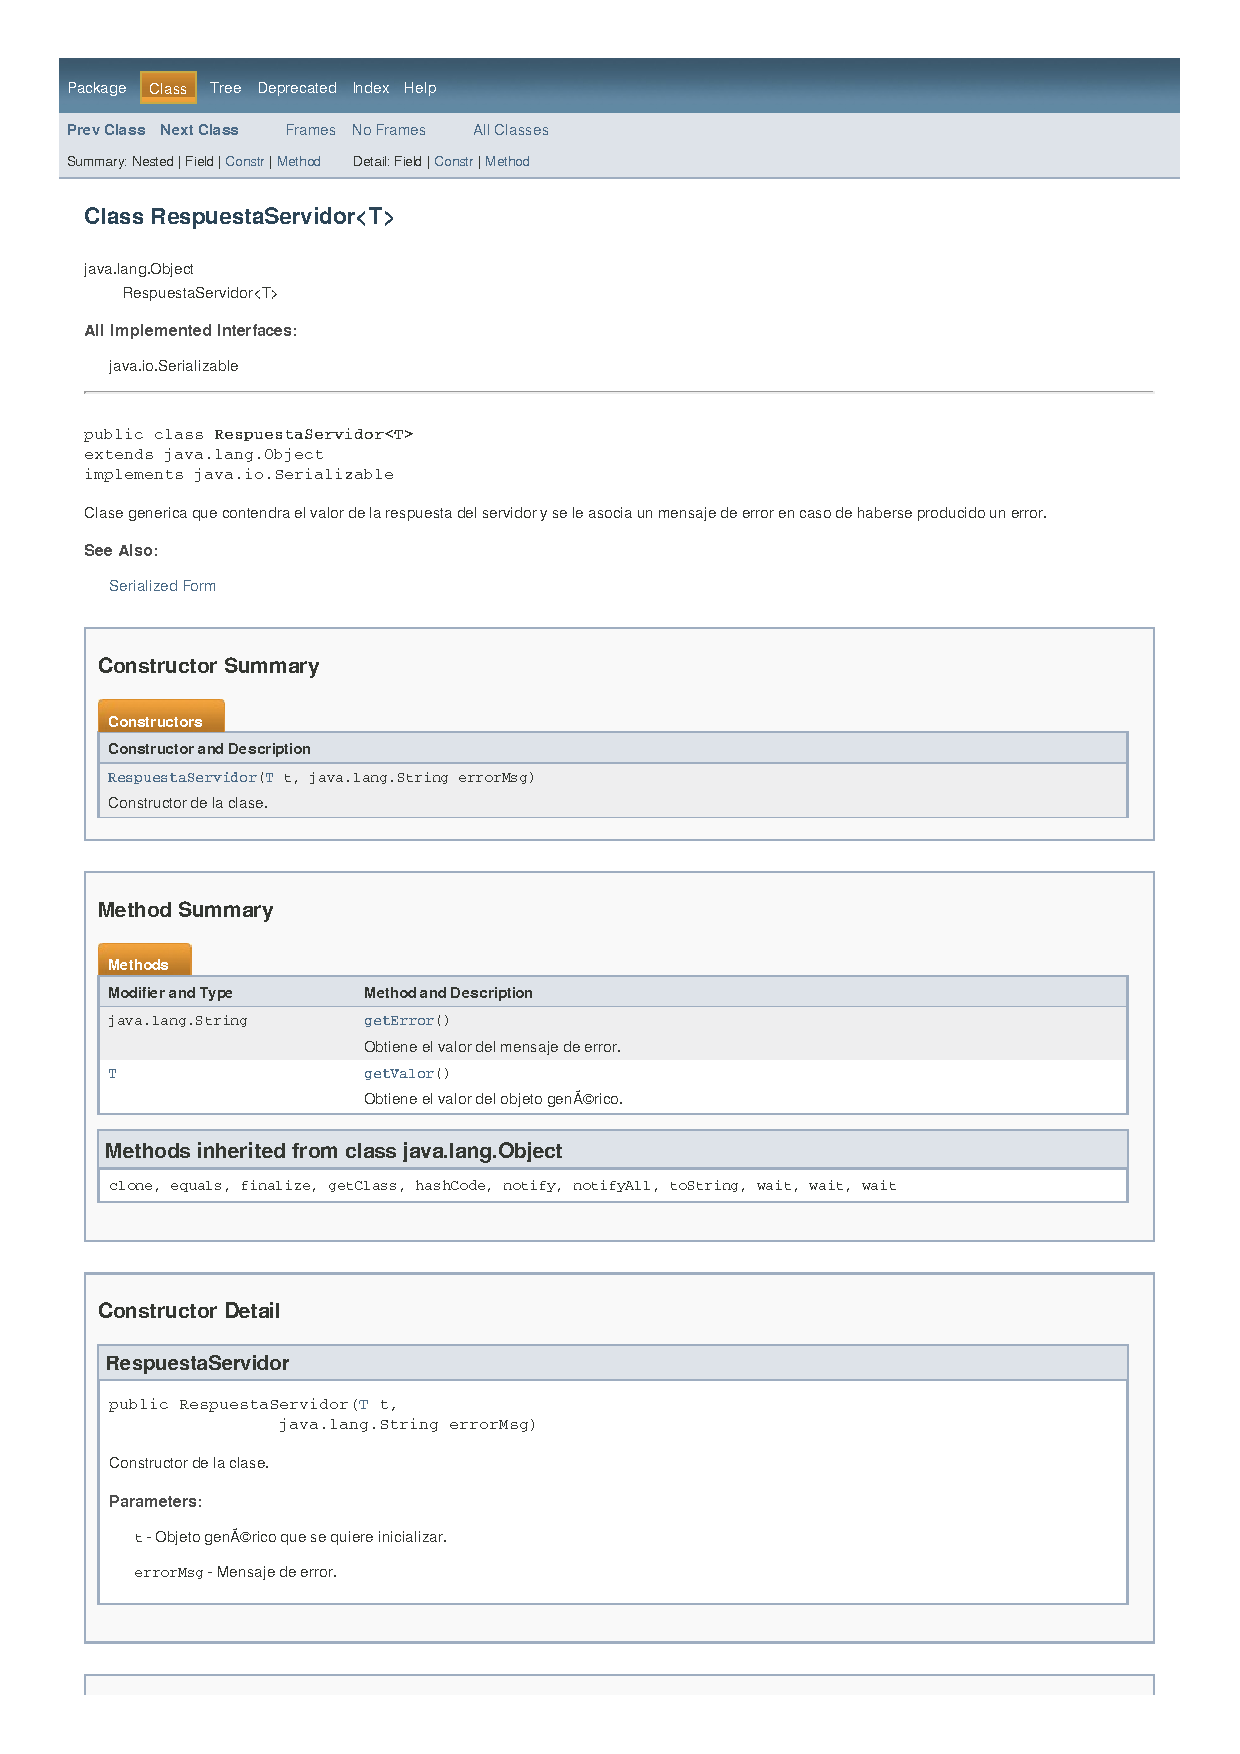
\includepdf[pages=-,nup=1x1,frame=false,scale=0.9,pagecommand={\label{doc:respuestaservidor}}]{javadoc/RespuestaServidor.pdf}
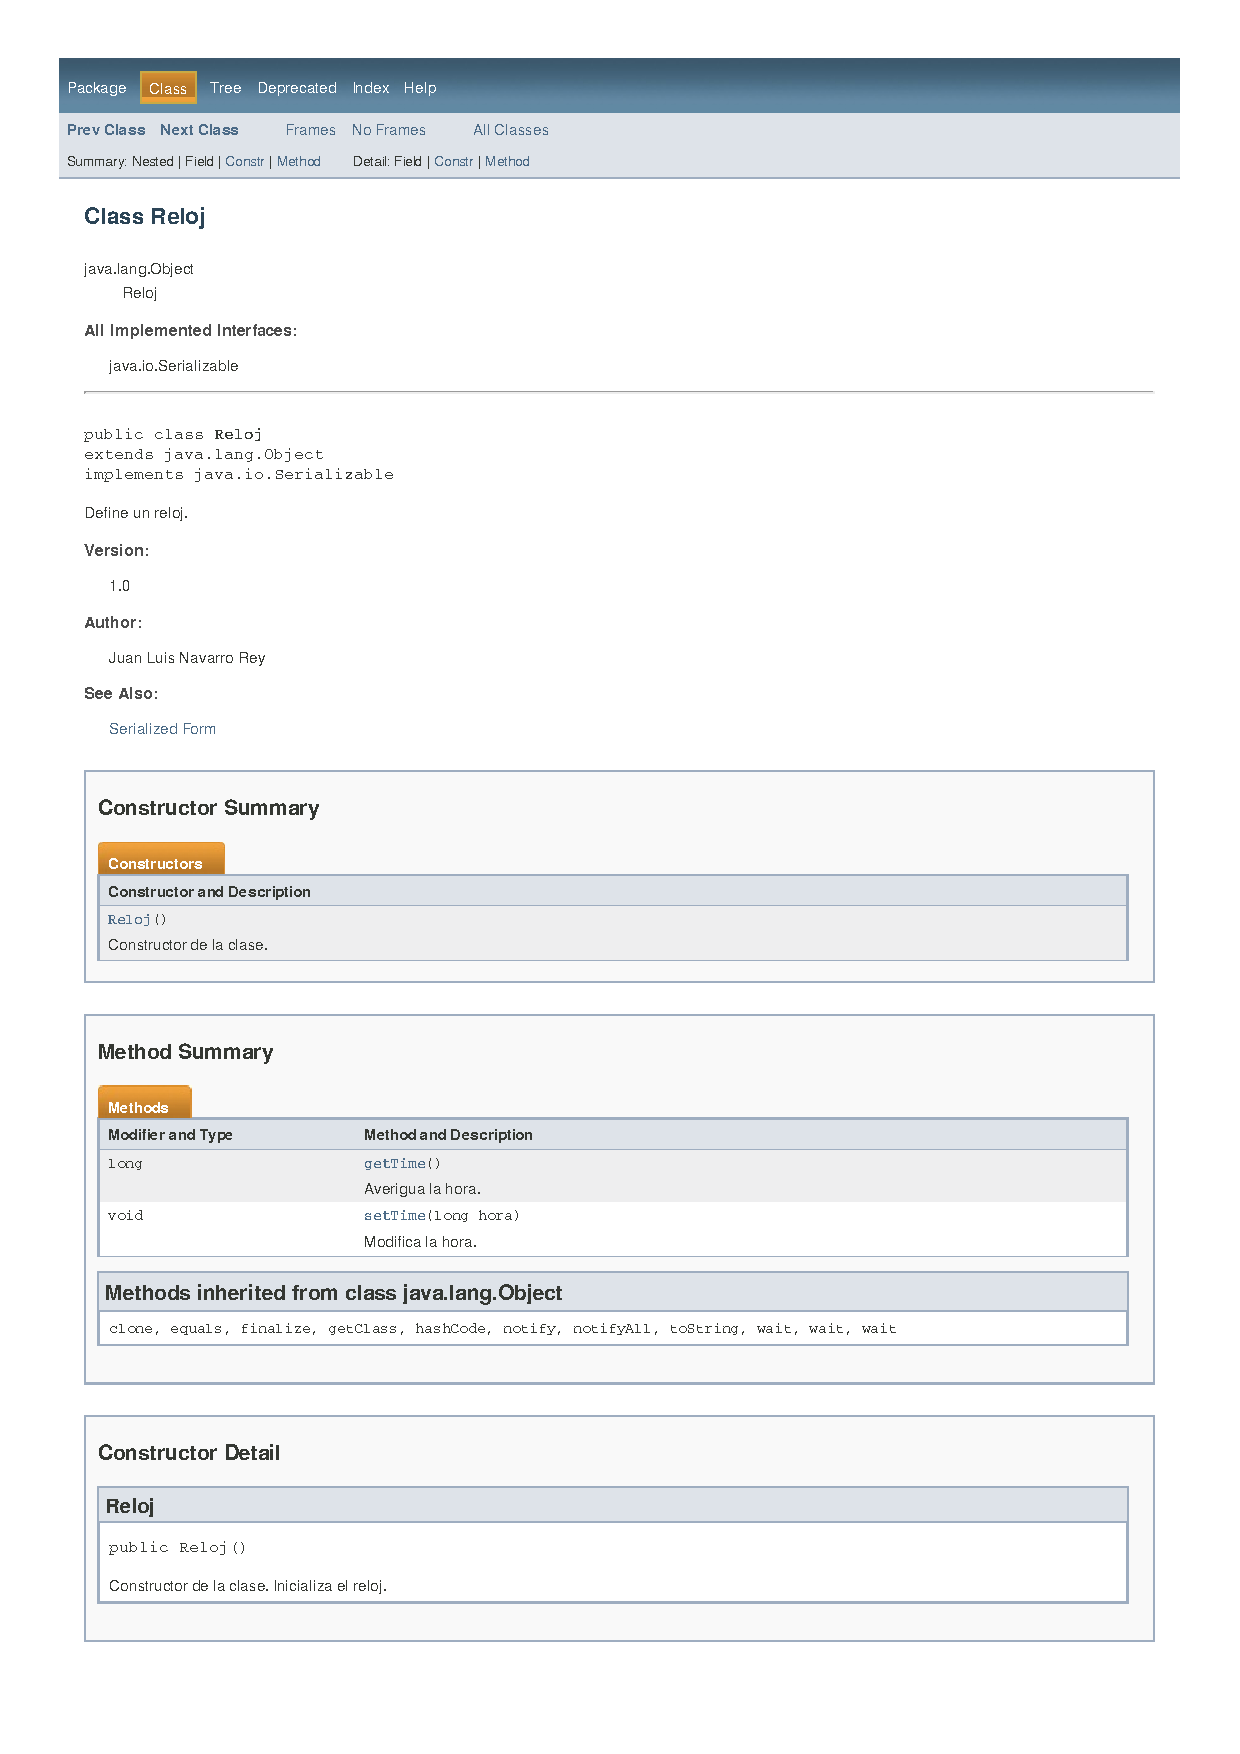
\includepdf[pages=-,nup=1x1,frame=false,scale=0.9,pagecommand={\label{doc:reloj}}]{javadoc/Reloj.pdf}
	
\end{document}